\chapter[DFT Errors]{DFT Errors, Convergence Failures and Repeat Calculations}
\label{chap:appendixdfterrors}


\subsection{Insufficient Memory}

The DFT calculations are performed on a supercomputer with many processors and many cores per processor.  The program uses two implementations of parallelization.

\begin{itemize}
\item OpenMP - many threads have access to the same shared memory
\item OpenMPI/MPICH - many processes, each with it's own memory
\end{itemize}

Whilst some favourable results have been shown using a hybrid of OpenMP and OpenMPI, it was more straightforward to use in OpenMPI mode only in this work.  Unfortunately, the amount of memory per process overwhelmed the computing nodes for certain calculations as each process requires an a copy of the data held in memory.  The job script was modified to reserve entire nodes and all the memory on each node, but to only use the cores on one of the two processors to halve the processes per node, but double the memory per process.  It was quicker to do this than wait in the high memory queue on BlueBEAR, where the memory per process would be perhaps double than that required.

\subsection{Scratch Restrictions}

When the calculations first started, the scratch space was located on a large shared space on the BlueBEAR computer.  Over time the drive space quota was restricted and the scratch was relocated to individual nodes.  There were few issues with less complex calculations as the \acrshort{scf} temporary data was several GB in size with the scratch space on each node being approximately 120GB.  Once a batch of collinear iron calculations had been submitted to the job queue, they would quickly fill the scratch drive and the job would terminate after just a few calculations, as the node had run out of scratch drive space.

\begin{lstlisting}[style=sBash,caption={Sbatch file},label={listing:sbatchfile}]
#!/bin/bash
#
#SBATCH --job-name=feforfit
#SBATCH --output=jobout.txt
#SBATCH --account=readmsd02
#
#SBATCH --ntasks 40
#SBATCH --nodes 1
#SBATCH --time 1800:00
#SBATCH --mem 180GB
#
#SBATCH --get-user-env
#SBATCH --export=NONE
#
unset SLURM_EXPORT_ENV

module purge; module load bluebear
module load bear-apps/2018a
module load iomkl/2018a
module load Python/3.6.3-iomkl-2018a
module load matplotlib/2.1.1-iomkl-2018a-Python-3.6.3

# Change to $PBS_O_WORKDIR
cd "$PBS_O_WORKDIR"
# Set the number of threads to 1
export OMP_NUM_THREADS=1
export PROC_COUNT=40
export PWSCF_SCRATCH=/scratch/bxp912
export PWSCF_PP=/rds/homes/b/bxp912/pp
export PWSCF_CACHE=/rds/homes/b/bxp912/pwscf_cache
export PWSCF_BIN=/rds/homes/b/bxp912/apps/qe-6.3/bin/pw.x
export PWSCF_SCRIPT=/rds/homes/b/bxp912/apps/qe-6.3/bin/pw.sh

python /rds/homes/b/bxp912/apps/python/qeforfit.py input.in > results.txt
\end{lstlisting}

\begin{lstlisting}[style=sBash,caption={Wrapper file},label={listing:wrapperfile}]
#!/bin/bash
rm -R $PWSCF_SCRATCH/*
mpirun -n $1 $PWSCF_BIN -in $2  > $3 
\end{lstlisting}

As the convergence and equation of state/elastic constant python programs automatically created and submitted the PWscf jobs, they would need to be continually restarted after clearing out the scratch.  To work around this a batch script (listing \ref{listing:sbatchfile}) and wrapper script (listing \ref{listing:wrapperfile}) for pw.sh were written.  The batch script sets the environment variables required for the sbatch job scheduling program and the wrapper script, and the wrapper script then clears the scratch directory before running PWscf.


\subsection{Caching Repeat Calculations}

Several of the programs required many hundreds of DFT calculations.  At first, if an error was encountered and the program had to start from scratch, computation time would be wasted.  To solve this, a directory was set to cache input and output files for PWscf.  A hash would be generated from the input file and this would be used as the cache file name.  If a calculation was successful, it would save the input and output file.  In future, if the same calculation was submitted again, the cached file would be returned.  The cache could be copied between BlueBEAR and other computers to save on repeat submission to the BlueBEAR job scheduler.



\subsection{Adjustment of DFT Parameters}

Throughout the DFT segment of this work, there were a number of issues that either resulted in the calculations failing or completing and not converging.  There were a number of causes for this and several solutions were used throughout the process to converge the \acrshort{scf} calculation.

Where the ecutwfc and ecutrho parameters are not converged there is a danger that values too low therefore containing too few plane waves in the basis set.  This might cause problems with the \acrshort{scf} causing it not to converge.  The same can be said about a failure to pick appropriate k-points and smearing.

There are a selection of mixing modes available in PWscf, giving a choice of Thomas-Fermi screening for homogeneous systems, local density dependent Thomas Fermi (local-TF) screening for inhomogeneous screening and Broyden mixing as the default.  

\begin{figure}[htb]
\centering
\begin{subfigure}{.49\textwidth}
  \centering
  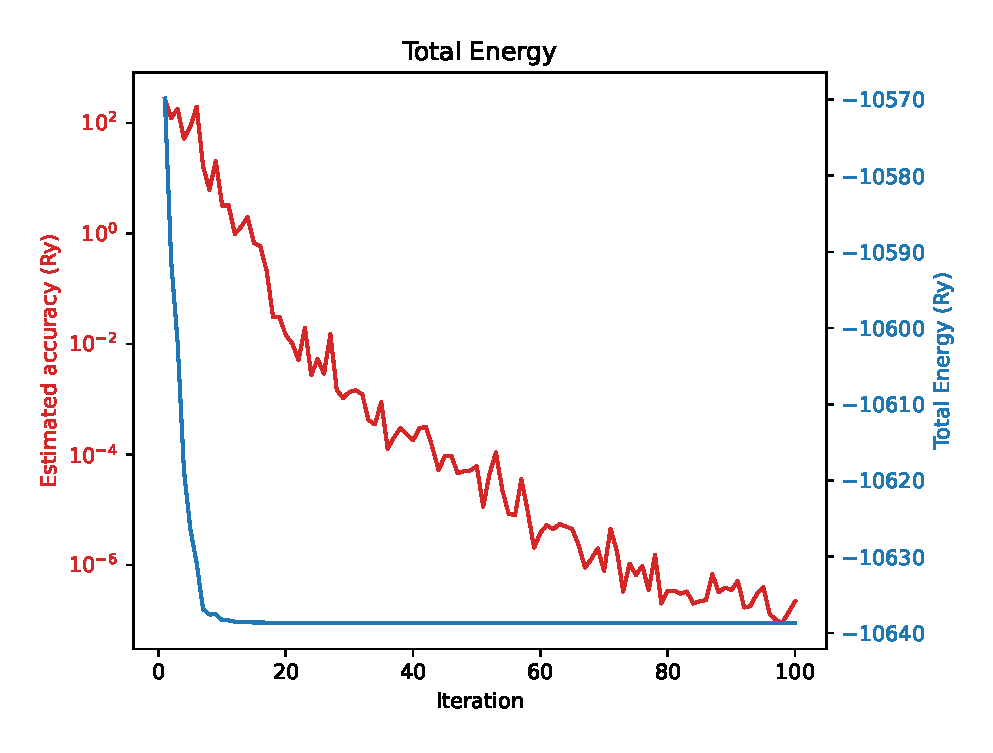
\includegraphics[width=.9\linewidth]{chapters/potentials_fe_pd_ru/convergence_failure/feru_1a_total_energy_0_plain.eps}
  \caption{Plain mixing failing to converge}
  \label{fig:feruplainmixing}
\end{subfigure}
\begin{subfigure}{.49\textwidth}
  \centering
  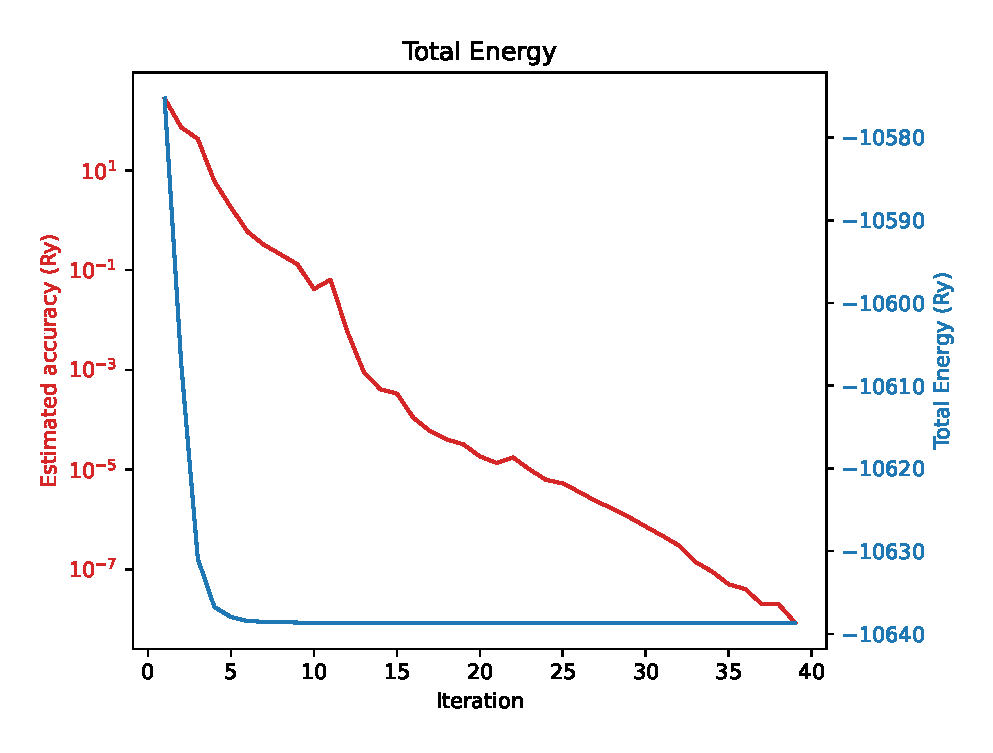
\includegraphics[width=.9\linewidth]{chapters/potentials_fe_pd_ru/convergence_failure/feru_1b_total_energy_0_local_tf.eps}
  \caption{Converging using local-TF mixing}
  \label{fig:ferulocaltfmixing}
\end{subfigure}
\caption{Fe-Ru calculations failed to converge in 100 iterations when plain mixing was used, but achieved convergence in under 40 iterations with local-TF convergence}
\label{fig:failuretoconverge}
\end{figure}

For calculations with defects the local-TF setting was used and for equation of state and elastic constant calculations, where the distribution of atoms is more homogeneous, plain Broyden mixing was used.  In most circumstances the mixing factor (mixing\_beta) was reduced to 0.1.  This wasn't always the case, and for certain defect calculations the default value of 0.3 proved to be the more efficient choice.

One other important parameter, that primarily affects geometry and position relaxation calculations (VC-RELAX), was the convergence threshold for the \acrshort{scf} calculations (conv\_thr).  The default value is $1.0\times 10^{-6}$ Ry and this was sufficient for \acrshort{scf} calculations and most VC-RELAX calculations.  Several relaxation calculations failed to converge and, at the suggestion of authors of Quantum Espresso, the threshold was reduced to $1.0\times 10^{-7}$ Ry.  This would lead to a longer time to compute the first geometry optimisation step.  The result from the first \acrshort{scf} cycle affects the convergence of subsequent steps and with the better starting point the time taken to complete the geometry relaxation was reduced and the chance of success was increased.



\subsection{Not Straying Too Far From Reality}

It is important to provide the calculation with reasonable and realistic configurations and settings.  Where a pure element such as Aluminium, Iron or Platinum was being investigated, the known experimental lattice parameters were used as a starting point (table \ref{table:predictedlattice} and table \ref{table:computedlattice}).  If the parameters were too far from these values, for example inputting a lattice parameter of either 2 or 8 angs for Aluminium rather than 4, as a starting approximation, the DFT calculation might struggle to relax the structure, or to even successfully run or converge a calculation.

The FCC Iron structure lattice parameter was estimated from the density of FCC steel, and the lattice parameter for alloys could similarly be estimated within a reasonable margin to use as a start point for the calculation.



\subsection{Trial Parameters for Iron with and Octahedral Defect}

Calculations where there is a high level of symmetry finished relatively quickly and without much trouble.  Where the position of each atom was perturbed slightly or where there was a defect the \acrshort{scf} calculations would take more iterations to converge and would often fail completely.  Where the geometry and atom position was also being optimised through repeated sets of \acrshort{scf} iterations the calculation would begin to converge but would ultimately fail through \acrshort{scf} non convergence.

\begin{table}[h]
\begin{center}
\begin{tabular}{c c c c c c c c c}
\hline\hline
Nbnd & Ntype & K & Degauss & Scfconv & Beta & Ndim & Mode & Iterations \\
\hline\hline
317 & 5 & 9x9x9 & 0.04 & $1.0 \times 10^{-6}$ & 0.1 & 10 & Plain & 75 \\
320 & 3 & 9x9x9 & 0.04 & $1.0 \times 10^{-6}$ & 0.05 & 10 & Local-TF & 46 \\
317 & 3 & 9x9x9 & 0.04 & $1.0 \times 10^{-7}$ & 0.1 & 10 & Local-TF & 42 \\
340 & 3 & 9x9x9 & 0.04 & $1.0 \times 10^{-6}$ & 0.8 & 8 & Local-TF & 38 \\
320 & 3 & 9x9x9 & 0.04 & $1.0 \times 10^{-6}$ & 0.1 & 10 & Local-TF & 36 \\
317 & 3 & 9x9x9 & 0.04 & $1.0 \times 10^{-6}$ & 0.8 & 8 & Local-TF & 33 \\
317 & 5 & 9x9x9 & 0.04 & $1.0 \times 10^{-6}$ & 0.3 & 8 & Local-TF & 32 \\
317 & 3 & 9x9x9 & 0.04 & $1.0 \times 10^{-6}$ & 0.3 & 8 & Local-TF & 32 \\
320 & 3 & 9x9x9 & 0.04 & $1.0 \times 10^{-6}$ & 0.3 & 10 & Local-TF & 29 \\
320 & 3 & 11x11x11 & 0.04 & $1.0 \times 10^{-6}$ & 0.3 & 10 & Local-TF & 29 \\
320 & 3 & 13x13x13 & 0.04 & $1.0 \times 10^{-6}$ & 0.3 & 10 & Local-TF & 29 \\
320 & 3 & 9x9x9 & 0.07 & $1.0 \times 10^{-6}$ & 0.3 & 10 & Local-TF & 25 \\
\hline\hline
\end{tabular}
\end{center}
\caption{Improving convergence SCF calculations of defects in Iron}
\label{table:trialparametersocta}
\end{table}

Iron with an octahedral defect was used to help fine tune parameters.  Initially a set of \acrshort{scf} calculations were performed with different parameters, and finally these were used to relax the cell geometry and atom positions for this defect.

Changing the number of k-points did not have an impact on the number of iterations required to converge, but changing the smearing value did.  An increase in smearing would be detrimental to the accuracy of convergence to the correct value and by doing this it would cause a difference in energy between past calculations with a smearing of 0.04Ry and and those with 0.07Ry.

The adjustment that had the largest impact on reducing the number of iterations was the change from plain mixing to Local-TF.  Following this, using a mixing beta of 0.3 where more weight is given to the previous state, also helped to reduce the number of iterations.

The attempts to optimise the values was not exhaustive as there were constrictions on time.  However, despite making these improvements and reducing the convergence threshold to $1.0 \times 10^{-8}$, the cell geometry and position relaxation of the starting configuration for an octahedral defect (by adding an atom at the octahedral location) also fails to relax by \acrshort{scf} non-convergence within an iteration of the relaxation algorithm. 

The optimization of the geometry and atom positions was likely due to it being a complex system to model with the initial configuration too far from the relaxed one.  To work around this the octahedral defect for a more simple metal, Aluminium, was relaxed to give a better starting point for the Iron calculation.  The increase in cell size was also applied.  With a better initial configuration and the adjusted parameters, the Iron octahedral calculation successfully completed.

This process was repeated for tetrahedral, 100, 110, 111 and crowdion defects.


